%
\documentclass[Proceedings]{ascelike}
%
% Feb. 14, 2013
%
% Some useful packages...
%
\usepackage{graphicx}
%\usepackage{subfigure}
%\usepackage{amsmath}
%\usepackage{amsfonts}
%\usepackage{amssymb}
%\usepackage{amsbsy}
%\usepackage{times}
%
%
% Place hyperlinks within the pdf file (works only with pdflatex, not latex)
% \usepackage[colorlinks=true,citecolor=red,linkcolor=black]{hyperref}
%
%
% NOTE: Don't include the \NameTag{<your name>} if you have selected 
%       the NoPageNumbers option: this leads to an inconsistency and
%       a warning, and the NameTag is ignored.
%\NameTag{Kuhn, Feb. 14, 2013}
%
%
\begin{document}
%
% You will need to make the title all-caps
\title{Determinaci\'on de la orbita de una estrella binaria espectrosc\'opica.}
%
\author{
Nicolas Garavito-Camargo%
%
% ---- The first of two styles for addresses: using footnotes and \thanks ----
\thanks{
Dept.\ de F\'isica.,
Universidad de los Andes, 
Calle 1...\ Bogot\'a, Colombia. E-mail: jn.garavito57@uniandes.edu.co}
\ Benjamin Oostra\footnotemark[1]
%
% Adding a second author with the same affiliation (still using \thanks):
%  \\
 %Colleague,\footnotemark[1] Member, ASCE%
%
% Adding another author with a different affiliation.  I have found that 
% the \and command doesn't quite work, so just use "and", as in the following 
% \\
% and
% Younyee Kuhn%
% \thanks{Flourishing wife of same.},%
% \ Not a Member, ASCE
%
% ---- The second of two styles for addresses: below names, no footnotes ----
%
% For this style, don't use \thanks.  Instead, use superscripts and carriage
% returns ("\\").  It's not pretty, but neither is the new ASCE proceedings
% style.  Something like the following:
%
% Matthew R. Kuhn$^1$, Member, ASCE\\[1ex]%
%
% $^1$\parbox[t]{5.75in}{Dept.\ of Civil Engrg.,
% Donald P.\ Shiley School of Engrg., Univ.\ of Portland, 
% 5000 N.\ Willamette Blvd., Portland, OR  97203. kuhn@up.edu.}
}
%
\maketitle
%
\begin{abstract}

\end{abstract}


%
% Some keywords, using a new command: \KeyWords{}
%
\KeyWords{..}
%
\section{Introducci\'on}


\subsection{Coordenadas ecuatoriales}

Las coordenadas astronomicas se utilizan para ubicar las estrellas en la bobeda celeste, 
En part\'icular las coordenadas ecuatoriales toman como punto referencia 
el punto vernal $\Upsilon$, 

\begin{figure}
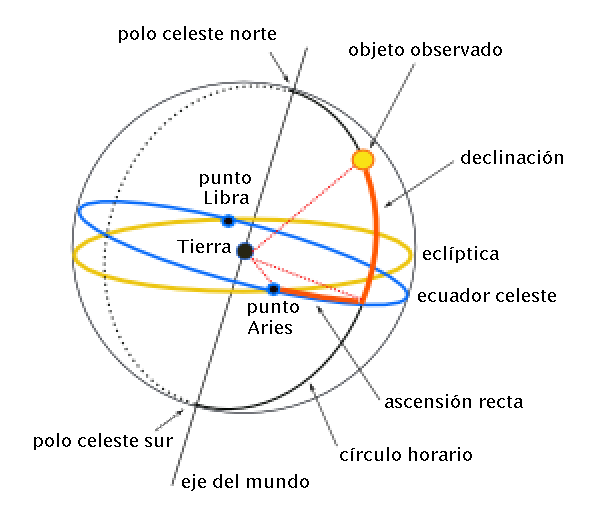
\includegraphics[scale=0.4]{Coordenadas_ecuatoriales.png}
\end{figure}

\subsection{Clasificacion espectral}

\section{Selecci\'on de la binaria a observar}

\section{Epsilon Coronae Australis}

Epsilon Coronae Australis ($\mathrm{\epsilon}$ CRA) ubicada en la 
constelcion de la Coronae Asutralis, es una binaria eclipsante \\

\begin{tabular}{c c}
\hline
Principales Caracteristicas\\
\hline
\hline
Asencion Recta & 18h58m43.5s \\
Declinacion & $-37^{0}$06'18'' \\
Periodo Orbital & 0.59 d\'ias \\
Magnitud & 4.83 \\
Clase espectral & F2 \\
Distancia entre estrellas & 2.9 Millones de Km\\ 
\hline
\hline
\end{tabular}

\begin{center}

\begin{figure}
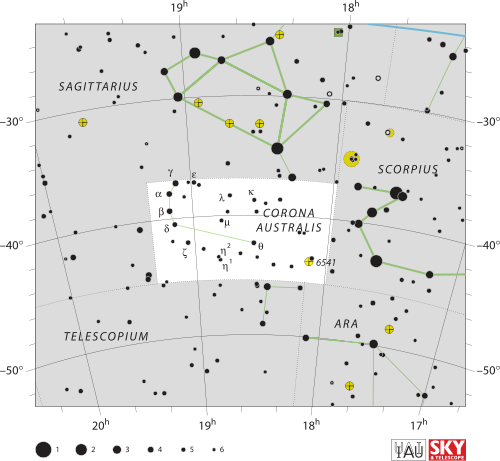
\includegraphics[scale=0.4]{CRA.png}
\caption{Corona Australis, http://www.iau.org/static/public/constellations/gif/CRA.gif \label{la}}
\end{figure}
\end{center}

\section{Observaciones}

Todas las observaciones se han llevado acabo en el observatorio astronomico de la 
Universidad de los Andes. A continuaci\'on se describen la instrumentacion utlizada
as\'i como los protocolos de observaci\'on utilizados.

\subsection{Instrumentaci\'on}

\subsubsection{Telescopio}

Se utilizo un telescopio marca Meade LX200 Schimdt-Cassegrain de $40 cm$ de apertura y una
distancia focal de $4m$

\begin{figure}
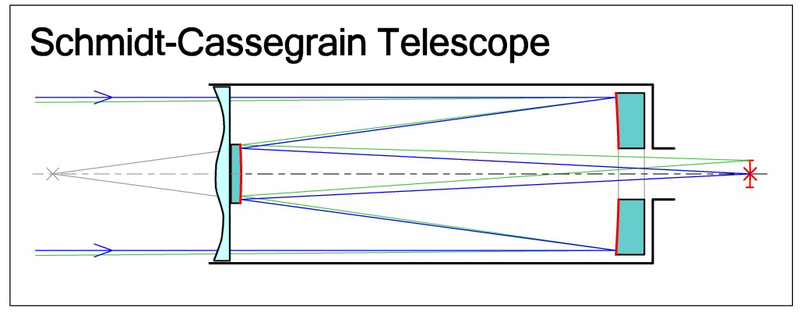
\includegraphics[scale=0.4]{SCT2.jpg}
\caption{Camino de luz en un telescopio Schmidt-Cassegrain, http://en.wikipedia.org/wiki/File:Schmidt-Cassegrain-Telescope.png \label{la}}
\end{figure}

\subsubsection{Espectrografo}

\subsubsection{Software}

\subsection{Protocolo de Observacion}

Todas las observaciones se han llevado acabo en un intervalo de tiempo aproximadamente 
desde las 5pm hasta las 9 pm.

\section{Resultados}

\section{References}

http://ned.ipac.caltech.edu

\end{document}
